\documentclass[a4,8pt]{article}
\usepackage[margin=3cm,includefoot]{geometry}
\usepackage{siunitx}
\usepackage{fancyhdr}
\usepackage{tikz}
	\usetikzlibrary{arrows,shapes,positioning,calc}
\usepackage[font=it]{caption}
\usepackage{amsmath}
\usepackage{float}

\pagestyle{fancy}
\lfoot{\sc Charlie Haddon}

\title{G484: Newtonian World}
\author{Charlie Haddon}

\begin{document}
\begin{titlepage}
	\pagenumbering{}
	\maketitle
	\vspace{15cm}
\end{titlepage}
\clearpage

\pagenumbering{arabic}

\section{General Motion}

\subsection{Newton's Laws of Motion}

Newton's three laws of motion are as follows:
\begin{enumerate}
	\item An object will remain at rest or move with constant velocity unless an external force acts upon it.
	\item The resultant force on an object is equal to its mass multiplied by its acceleration; $F=ma$ for constant mass.
	\item When a body exerts a force on another body, the second body simultaneously exerts an equal and opposite force on the original body.
\end{enumerate}


and some definitions of physical quantities:
\begin{itemize}
	\item Linear momentum, $p$ (\si{\kilo\gram\metre\per\square\second}), is defined as the product of the mass and velocity of an object and is a vector quantity.
	\item Net force, $F$ (\si{\newton}), on a body is equal to the rate of change of its momentum, $F=\frac{dp}{dt}$ or if the force is approximately constant, $F \approx \frac{\Delta p}{\Delta t}$
	\item Impulse, $J$ (\si{\newton\second}), is the integral of force over time or for constant force; force multipied by time and is therefore equal to the change in momentum, $mv-mu$.
\end{itemize}


\subsection{Collisions}
The principle of conservation of momentum states that the momentum of a system remains constant if no external force acts upon it. This princible is invaluable for calculating the velocities and masses in an n-body collision. For example, in a collision involving 2 bodies, $A$ and $B$:
$$m_A u_A + m_B u_B = m_A v_A + m_B v_B$$

\begin{figure}[H]
\begin{center}
Before collision:\\
\vspace{0.25cm}
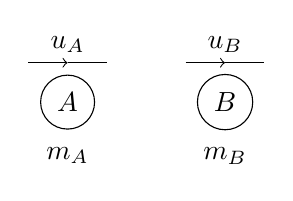
\begin{tikzpicture}[scale=1]
	\node[circle,draw] at (1,1) (A) {$A$};
	\node[below=0.1 of A] (1,1) {$m_A$}; 
	\draw[->] (0.5,1.5) -- (1,1.5) node[above] {$u_A$};  
	\draw (1,1.5) -- (1.5,1.5);

	\node[circle,draw] at (3,1) (B) {$B$};
	\node[below=0.1 of B] (3,1) {$m_B$}; 
	\draw[->] (2.5,1.5) -- (3,1.5) node[above] {$u_B$};  
	\draw (3,1.5) -- (3.5,1.5);
\end{tikzpicture}
\\
\vspace{0.5cm}

After collision:\\
\vspace{0.25cm}
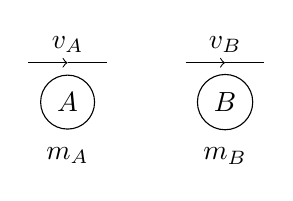
\begin{tikzpicture}[scale=1]
	\node[circle,draw] at (1,1) (A) {$A$};
	\node[below=0.1 of A] (1,1) {$m_A$}; 
	\draw[->] (0.5,1.5) -- (1,1.5) node[above] {$v_A$};  
	\draw (1,1.5) -- (1.5,1.5);

	\node[circle,draw] at (3,1) (B) {$B$};
	\node[below=0.1 of B] (3,1) {$m_B$}; 
	\draw[->] (2.5,1.5) -- (3,1.5) node[above] {$v_B$};  
	\draw (3,1.5) -- (3.5,1.5);
\end{tikzpicture}
\caption{Two objects collide and separate}
\end {center}
\end{figure}

or if the objects coalesce to form a single object, $C$:
$$m_A u_A + m_B u_B = (m_A + m_B) v_C$$

\begin{figure}[H]
\begin{center}
Before collision:\\
\vspace{0.25cm}
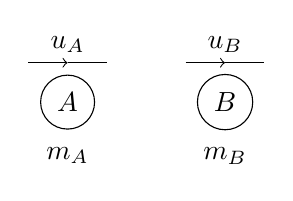
\begin{tikzpicture}[scale=1]
	\node[circle,draw] at (1,1) (A) {$A$};
	\node[below=0.1 of A] (1,1) {$m_A$}; 
	\draw[->] (0.5,1.5) -- (1,1.5) node[above] {$u_A$};  
	\draw (1,1.5) -- (1.5,1.5);

	\node[circle,draw] at (3,1) (B) {$B$};
	\node[below=0.1 of B] (3,1) {$m_B$}; 
	\draw[->] (2.5,1.5) -- (3,1.5) node[above] {$u_B$};  
	\draw (3,1.5) -- (3.5,1.5);
\end{tikzpicture}
\\
\vspace{0.5cm}

After collision:\\
\vspace{0.25cm}
\begin{tikzpicture}[scale=1]
	\node[circle,draw] at (1,1) (C) {$C$};
	\node[below=0.1 of A] (m) {$m_A + m_B$}; 
	\draw[->] (0.5,1.5) -- (1,1.5) node[above] {$v_C$};  
	\draw (1,1.5) -- (1.5,1.5);
\end{tikzpicture}
\caption{Two objects collide and coalesce}
\end{center}
\end{figure}

In a perfectly elastic collision, both momentum and kinetic energy are conserved, whereas in an inelastic collision, only momentum is conserved as some kinetic energy is lost to things like heat and sound etc.

\section{Circular Motion and Oscillations}
\subsection{Circular Motion}
A radian is the natural unit for measuring angles. A radian is defined as the angle subtended at the centre of a circle by an arc length equal to the circle's radius. One radian is equal to $\frac{180}{\pi}$ degrees.

\begin{figure}[H]
\begin{center}
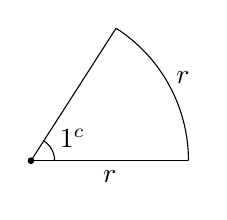
\begin{tikzpicture}
	\filldraw[black] (0,0) circle (1pt);
	\draw (0,0) -- (2,0);
	\draw (0,0) -- (1r:2);
	\draw (2,0) arc (0:1r:2);
	\draw (0.3,0) arc (0:1r:0.3);

	\node (theta) at (0.5r:0.6) {$1^c$};
	\node (r1) at (1,-0.2) {$r$};
	\node (r2) at (0.5r:2.2) {$r$};
\end{tikzpicture}
\caption{One radian}
\end{center}
\end{figure}

Circular motion is the result of a force acting perpendicular to an object's velocity, keeping the object at a fixed distance, $r$, from the origin. The general term for this force is centripetal force. An object undergoing circular motion is not in equilibrium as the resultant force is towards the centre of the circle, therefore the object is also accelerating towards the centre of the circle (centripetal acceleration). The speed of such an object is equal to $\frac{2\pi r}{T}$ where $r$ is the radius of the motion and $T$ is the time period (the time taken to complete a full cycle). The cetripetal acceleration is equal to $\frac{v^2}{r}$ where $v$ is the linear velocity calculated as before. Therefore, by Newton's second law, $F=ma$, centripetal force is equal to $\frac{mv^2}{r}$.

\begin{figure}[H]
\begin{center}
\begin{tikzpicture}
	\filldraw[black] (0,0) circle (1pt) node[below] {$O$};
	\draw[dashed] (60:2) arc (60:360:2);
	\draw (0:2) arc (0:60:2);
	\draw (0:2) -- (60:2);
	\node at ($(2,0) + (120:1) - (30:0.3)$) {$s$};
	\draw (0:0.3) arc (0:60:0.3);
	\node (theta) at (30:0.6) {$\delta\theta$};

	\draw (0,0) -- (2,0);
	\node at (1,-0.2) {$r$};
	\filldraw[black] (2,0) circle (1pt);
	\draw[->] (2,0) -- (2,1);
	\node at (2.3,0.5) {$v_0$};

	\draw (0,0) -- (60:2);
	\node at ($(60:1) + (150:0.2)$) {$r$};
	\filldraw[black] (60:2) circle (1pt);
	\draw[->] (60:2) -- ++(150:1);
	\node at ($(60:2) + (150:0.5) + (60:0.3)$) {$v_1$};
\end{tikzpicture}
\caption{Deriving the equation for centripetal acceleration}
\end{center}
\end{figure}

\subsection{Gravitational Fields}
A gravitational field is produced by all bodies with mass. By Newton's law of gravitation: Two bodies with mass exert a force on eachother proportional to the product of their masses and inversely proportional to the square of the distance between them. Gravitational field strength, $g$ (\si{\newton\per\kilo\gram}), is a measure of the force exerted on an object by a gravitational field per unit mass. Gravitational fields can be graphically represented using field lines showing the sources of gravitational field.

\begin{figure}[H]
\begin{center}
\begin{tikzpicture}
	\node[draw,circle] (O) at (0,0) {$m$};
	\foreach \theta in {0,45,90,135,180,225,270,315}
	{
		\draw (O) -- (\theta:1);
		\draw[->] (\theta:2) -- (\theta:1);
	}
\end{tikzpicture}
\caption{Gravitational field around a massive body}
\end{center}
\end{figure}

The constant of proportionality that relates gravitational force to mass and distance is $G$ and the equation for the force between two spherical or point masses is $F=-\frac{GMm}{r^2}$ where $M$ and $m$ are the masses of the two bodies and $r$ is the distance between them. By dividing throughout by one of the mass terms, the equation also gives the gravitational field strength of a point with distance $r$ from a mass: $g=-\frac{GM}{r^2}$. For large bodies like the Earth the gravitational field strength at the surface is approximately uniform. For the Earth this value is approximately equal to 9.81\si{\meter\per\square\second} (acceleration of free fall).

For an oscillating object or object in circular motion the time taken to complete a full cycle of motion is called a period. Kepler found by observation that that for all the planets in the solar system $T^2 \propto r^3$ where $T$ is the period of the planet's orbit and $r$ is its distance from Earth. This equation works only for objects in circular orbits and is dervied thusly:

By equating gravitational force and centripetal force:
$$\frac{GMm}{r^2} = \frac{mv^2}{r}$$

Dividing through by $m$ and multiplying by $r^2$:
$$GM = rv^2$$

Substituting in $v = \frac{2 \pi r}{T}$:
$$GM = r\left(\frac{2 \pi r}{T}\right)^2$$
$$\implies GM = \frac{4 {\pi}^2 r^3}{T^2}$$

And finally, rearranging for $T^2$:
$$T^2 = \left(\frac{4 {\pi}^2}{GM}\right)r^3$$

As $\frac{4 {\pi}^2}{GM}$ is constant:
$$T^2 \propto r^3$$

Satellites that orbit the Earth about the equator with a period of one day are called geostationary because they remain directly above the same point on the Earth at all times and are therefore stationary relative to Earth. This is particularly useful for communication satellites as it provides reliable coverage of a specific area meaning antannae don't need to track them and can be produced and maintained much more cheaply.

\subsection{Simple Harmonic Oscillations}
Simple harmonic motion is a type of motion where an object oscillates with a restorative force proportional to the object's displacement from an equilibrium position and in the opposite direction. Some objects in the physical world oscillate in a way that approximates simple harmonic motion. Examples include pendulums and masses hanging from springs. The course requires that one can define certain terms relating to SHM:
\begin{itemize}
	\item Displacement is the vector distance between two objects. For example: between the equilibrium point and an object undergoing SHM.
	\item Amplitude with regards to SHM is the maximum displacement of the oscillating object from the equilibrium point.
	\item The period of an oscillation is the time between two identical points in the cycle, most commonly the points at which the oscillating object has zero displacement and positive velocity.
	\item Frequency is the inverse of period i.e. the number of full oscillations per unit time.
	\item Angular frequency is the magnitude of the vector quantity angular velocity (angular displacement per unit time) or $\frac{2\pi}{T}$ for objects in circular motion.
	\item Phase difference is the amount two sinusoidal functions are offset from eachother, measured in radians.
\end{itemize}

The defining equation of simple harmonic motion is $a=-(2\pi f)^2 x$ as acceleration is proportional to displacement, $x$, with the constant of proportionality $-(2\pi f)^2$ where $f$ is the frequency of the oscillation. $2\pi f$ is angular frequency often reffered to by the letter $\omega$. Some other important equations for SHM are general solutions to the previous differential equation: $x=Acos\omega$ and $x=Asin\omega$. Therefore the maximum velocity of the oscillating object is given by: $v_\text{max}=\omega A$. It should be noted that the amplitude scales the function only in the $x$ direction and the scale in the $t$ direction remains the same. This means that the amplitude of the oscillation does not change the frequency or period.
\vspace{8pt}

The relationships between time and displacement, velocity and acceleration for simple harmonic motion where $x=Asin\omega$ ($x=sint$: $\dot{x}=cost$ and $\ddot{x}=-sint$):
\begin{figure}[H]
\begin{center}
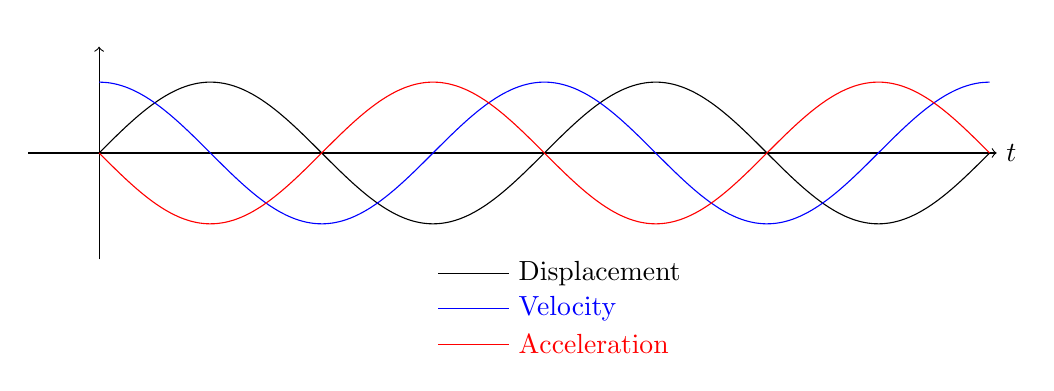
\begin{tikzpicture}[scale=0.9]
	\draw[->] (-1,0  ) -- (4*pi+0.1,0) node[right] {$t$};
	\draw[->] (0,-1.5) -- (0,1.5     ) node[above] {};

	\draw[smooth,samples=100,domain=0:4*pi,variable=\t,black] plot ({\t},{sin(deg(\t))});
	\draw[smooth,samples=100,domain=0:4*pi,variable=\t,blue ] plot ({\t},{cos(deg(\t))});
	\draw[smooth,samples=100,domain=0:4*pi,variable=\t,red  ] plot ({\t},{-sin(deg(\t))});
	
	\draw[black ] (2*pi-1.5,-1.7) -- (2*pi-0.5,-1.7) node[right] {Displacement};
	\draw[blue  ] (2*pi-1.5,-2.2) -- (2*pi-0.5,-2.2) node[right] {Velocity};
	\draw[red   ] (2*pi-1.5,-2.7) -- (2*pi-0.5,-2.7) node[right] {Acceleration};
\end{tikzpicture}
\end{center}
\caption{Simple harmonic motion}
\end{figure}

As an object oscillates between displacements of $-A$ and $A$, potentital energy is converted into kinetic energy and vice versa. When the object's displacement is equal to $\pm A$ it has maximum potential energy and zero kinetic energy. As the object returns to the equilibrium point where dispacement is zero, its potential energy  is converted into kinetic energy until it reaches maximum kinetic energy and zero potential energy. As the object moves from the equilibrium point the kinetic energy is again converted into potential energy as the object approaches $\mp A$. The kinetic energy is proportional to the square of the velocity and the potential energy could be gravitational potential energy or elastic potential energy etc. 
Damping creates exponential decay in the oscillators sinusoidal motion causing the amplitude of the motion to reduce with time.

\begin{figure}[H]
\begin{center}
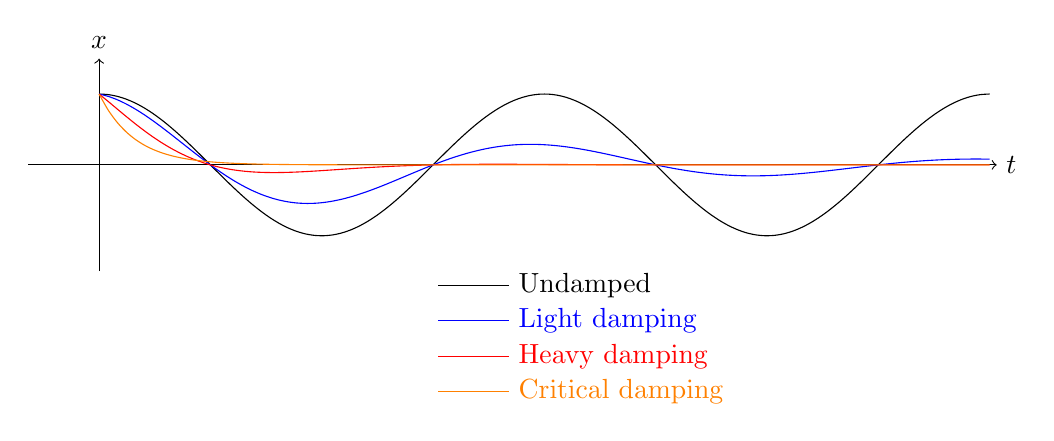
\begin{tikzpicture}[scale=0.9]
	\draw[->] (-1,0  ) -- (4*pi+0.1,0) node[right] {$t$};
	\draw[->] (0,-1.5) -- (0,1.5     ) node[above] {$x$};
	\draw[smooth,samples=100,domain=0:4*pi,variable=\t,black ] plot ({\t},{cos(deg(\t))});
	\draw[smooth,samples=100,domain=0:4*pi,variable=\t,blue  ] plot ({\t},{exp(-0.2*\t)*cos(deg(\t))});
	\draw[smooth,samples=100,domain=0:4*pi,variable=\t,red   ] plot ({\t},{exp(-0.8*\t)*cos(deg(\t))});
	\draw[smooth,samples=100,domain=0:4*pi,variable=\t,orange] plot ({\t},{exp(-2*\t)});

	\draw[black ] (2*pi-1.5,-1.7) -- (2*pi-0.5,-1.7) node[right] {Undamped};
	\draw[blue  ] (2*pi-1.5,-2.2) -- (2*pi-0.5,-2.2) node[right] {Light damping};
	\draw[red   ] (2*pi-1.5,-2.7) -- (2*pi-0.5,-2.7) node[right] {Heavy damping};
	\draw[orange] (2*pi-1.5,-3.2) -- (2*pi-0.5,-3.2) node[right] {Critical damping};
\end{tikzpicture}
\end{center}
\caption{Damped oscillation}
\end{figure}

The principles of oscillations and resonance are utilised in musical instruments and various other apparatus. Forced oscillations are used in speakers. Objects have a natural frequency based on their physical properties at which they will oscillate with the greatest amplitude (resonance). This has to be considered when constructing buildings and bridges because vibrations that have almost the same frequency as the natural frequency of the contruction can cause oscillations with large amplitude resulting in structural failure and collapse.

\begin{figure}[H]
\begin{center}
\begin{tikzpicture}
	\draw[->] (0,0) -- (3*3.1,0) node[right] {$f$};
	\draw[->] (0,0) -- (0,6) node[above] {$A$};
	\draw[smooth,samples=100,domain=0:3,variable=\f,black] plot ({\f*3},{1/(sqrt((1-\f^2)^2+(0.1*2*\f)^2))});
	\draw[smooth,samples=100,domain=0:3,variable=\f,blue ] plot ({\f*3},{1/(sqrt((1-\f^2)^2+(0.2*2*\f)^2))});
	\draw[smooth,samples=100,domain=0:3,variable=\f,red  ] plot ({\f*3},{1/(sqrt((1-\f^2)^2+(0.3*2*\f)^2))});

	\filldraw[black] (3,0  ) circle (1pt) node[below] {$f_0$};
	\filldraw[black] (1.5,0) circle (1pt) node[below] {$\frac{1}{2}f_0$};
	\filldraw[black] (6,0  ) circle (1pt) node[below] {$2f_0$};

	\draw[black] (1.5*3.1-1.5,-0.7) -- (1.5*3.1-0.5,-0.7) node[right] {Undamped};
	\draw[blue ] (1.5*3.1-1.5,-1.2) -- (1.5*3.1-0.5,-1.2) node[right] {Light damping};
	\draw[red  ] (1.5*3.1-1.5,-1.7) -- (1.5*3.1-0.5,-1.7) node[right] {Heavy damping};
\end{tikzpicture}
\end{center}
\caption{Forced oscillation}
\end{figure}

\section{Thermal Physics}
\subsection{States of Matter}
Kinetic theory describes substances as structures comprised of particles (atoms, molecules, etc.) with various kinetic energies. Classical kinetic theory allows matter to exist in a solid, liquid or gaseous state.

\begin{itemize}
	\item Properties of solids:
		\begin{itemize}
			\item Regular three-dimensional structure.
			\item Particles are bonded together by strong electrostatic attraction.
			\item There is little space between particles.
			\item Particles oscillate in simple harmonic motion about fixed positions.
			\item Heating increases the kinetic energy of the particles resulting in increased amplitude of oscillation.
			\item If the particles are heated so that they are able to break free of their bonds, the heat energy is converted to potential energy and the solid melts.
		\end{itemize}
	\item Properties of liquids:
		\begin{itemize}
			\item Particles remain in contact but are free to move liquids, therefore, have no fixed shape.
			\item The separation of particles is about the same as in a solid.
			\item Increasing the temperature of a liquid increases the kinetic energy of the molecules until they are able to break free from eachother (vaporisation).
		\end{itemize}
	\item Properties of gases:
		\begin{itemize}
			\item Intermolecular forces are negligible so the dominant force is the reaction when particles collide with the walls of the container.
			\item Particles are about ten times further apart than in solids or liquids.
			\item Heating a gas causes an increase in the kinetic energy and speed of particles.
		\end{itemize}
\end{itemize}

Particles in liquids and gases appear to move randomly, frequently changing direction. This is called Brownian motion after botanist Robert Brown who observed this motion with pollen grains suspended in water. The motion can be explained using kinetic theory and its effect can be demonstrated using a smoke cell and a microscope. A glass cell is filled with smoke and placed under a low-power microscope and a light is shone on the cell from the side. One may remove the eyepiece and replace it with a video camera to record the effect. The smoke particles travel in a direction at a fairly constant speed then spontaneously change direction and continue to travel at approximately the same speed. The effect can be explained by considering a single smoke particle. The smoke particle is very large compared to the surrounding air molecules which are colliding with it at random. At any given moment the particle has a net force in a particular direction because the vector sum of the impacts has a particular direction because there is an imbalance in the number of molecules colliding with each side of the smoke particle. Thus the particles appears to have a random 'jerky' motion.

The pressure of a gas is the force exerted per unit area of its container, $p=\frac{F}{A}$ (\si{\newton\per\square\meter} or \si{\pascal}). Pressure of a gas can be explained in terms of particles using kinetic theory assuming that:

\begin{itemize}
	\item Collisions between the particles and the walls are perfectly elastic.
	\item The time of a collision is negligible compared to the time between collisions.
	\item The size of the molecules is negligible compared to the size of the container.
	\item Intermolecular forces are negligible except during collisions.
	\item The gravitational force is negligible.
\end{itemize}

Consider a gas inside a container: Particles of the gas move randomly and collide with the walls. When a gas particle collides with a wall its momentum is flipped in the direction of the normal to the surface and therefore a force is exerted on the wall. Because the number of molecules is large, the net force exerted on the walls is measureable and approximately uniform.

\begin{figure}[H]
\begin{tikzpicture}
\end{tikzpicture}
\caption{Kinetic pressure model}
\end{figure}

The internal energy of a substance is the sum of the random distribution of the kinetic and potential energies of its particles. The internal energy of a substance continuously increases as it is heated. Consider a solid that is being heated at a constant rate. The temperature increase first contributes to the kinetic energy, increasing the amplitude of the particles' vibrations until the solid reaches its melting point. Now the thermal energy is used to break the bonds holding the particles together, increasing the potential enrgy while the kinetic energy remains constant. The solid then melts to form a liquid and follows similar behaviour as it heats until it evaporates. Thermal energy is distinct from internal energy and is defined as the energy transferrred between two points as a result of a temperature difference betweeen them. The internal energy of a system is increased by supplying thermal energy or doing work on the system and reduced by transferring thermal energy away from the system or letting the system do work on the surroundings.

\begin{figure}[H]
\begin{center}
\begin{tikzpicture}
	\draw[->] (0,0) -- (6,0) node[right] {$E$};
	\draw[->] (0,0) -- (0,4) node[above] {$\theta$};

	\draw (0,0) -- (1,1) -- (2,1) -- (3,2) -- (4,2) -- (5,3);
\end{tikzpicture}
\caption{Temperature during state changes}
\end{center}
\end{figure}

Consider a cylinder full of air sealed by a piston. Supplying heat to the cylinder whilst the piston remains stationary causes an increase in the kinetic and internal energies of the air. Depressing the piston does work on the air, increasing the potential and internal energies of the air. The temperature changes with the kinetic energy of the particles.

Liquids can evaporate at temperatures lower than their boiling point. This is due to the distribution of molecules with various kinetic energies. Molecules with higher energy may escape from the surface of the liquid. The rate of evaporation is modified by the temperature of the liquid, the surface area of the liquid and the rate at which the escaped particles are carried away (e.g. surface airflow).

\begin{figure}[H]
\begin{center}
\begin{tikzpicture}
\end{tikzpicture}
\end{center}
\caption{Evaporation}
\end{figure}

\subsection{Temperature}
On average, thermal energy is transferred from regions of higher temperature to regions of lower temperature; for two objects $A$ and $B$, if $T_A>T_B$, there is a net flow of thermal energy from $A$ to $B$. Therefore the temperature of $A$ decreases and the temperature of $B$ increases until they are equal. When the rate of transfer of heat energy from $A$ to $B$ equals the rate of transfer of heat energy from $B$ to $A$, $A$ and $B$ have reached thermal equilibrium. Temperature is the property which determines whether or not an object is in thermal equilibrium with another.

There are various temerature scales in use today, all of which are based on two fixed points:

\begin{itemize}
	\item The Celsius scale:
		\begin{itemize}
			\item Measured in degrees Celsius (\si\celsius).
			\item The fixed points are the freezing point of water (0\si\celsius) and the boiling point of water (100\si\celsius).
		\end{itemize}
	\item The thermodynamic (Kelvin, absolute) scale:
		\begin{itemize}
			\item Measured in Kelvin (\si\kelvin).
			\item The fixed points are absolute zero (0\si\kelvin) and the triple point of water (273.16\si\kelvin). 
		\end{itemize}
\end{itemize}

The Kelvin scale is the most widely used in science today because it is absolute. That is, it is based on a fundamental property of the universe (absolute zero, minimalinternal energy) rather than a property of a particular material. Absolute zero is calculated theroetically using the idea of a 'perfect heat engine'. The pressure of a fixed mass of gas in a sealed container of fixed volume is found to decrease as the teperature is reduced. This behaviour can be extrapolated to find the temperature of a gas that exerts zero pressure on its container: -273\si\celsius. Absolute temerature tends to be represented by the symbol $T$ where degrees of temerature are represented by $\theta$.

$$T(\si\kelvin) = \theta(\si\celsius) + 273.15$$

\subsection{Thermal Properties of Materials}
The change in teperature of an object is influnced by:

\begin{itemize}
	\item The heat energy supplied to the object, $\Delta\theta \propto E$.
	\item The mass of the object, $\Delta\theta \propto \frac{1}{m}$.
	\item The heat capacity of the object.
\end{itemize}

The specific heat capacity, $c$ (\si{J kg^{-1} K^{-1}}) of a substance is the amount of energy required to raise the temperature of 1\si{\kilogram} of the substance by 1\si{\kelvin} assuming no change of state. The energy required to produce a certain temperature change is given by:

$$E = mc \Delta T$$ 

There is a simple method to measure the specific heat capacity of a solid. 

\begin{figure}[H]
\begin{tikzpicture}
\end{tikzpicture}
\caption{An experiment to measure specific heat capacity}
\end{figure}

Latent heat is the heat energy that a body will absorb or givve out when changing state. The heat produced by a substance changing from liquid to solid with no temperature change is called latent heat of fusion and the heat required to change a substance from liquid to gas with no change in temperature is called lantent heat of vaporisation. The specific latent heat of fusion (or vaporisation) of a substance is the energy required to change 1\si{\kilogram} of the substance from solid to liquid (or liquid to gas) at constant temperature.

$$E = ml$$

\subsection{Ideal Gases}
Boyle's law states that the pressure of a fixed mass gas at constant temperature is inversely proportional to its volume, $p \propto \frac{1}{V}$, and pressure multiplied by volume is constant, $p_1 V_1 = p_2 V_2$. Charles' law states that volume is proportional to temperature for constant pressure, $V \propto T$. The pressure law states that the pressure of a fixed mass gas is directly proportional to its absolute temperature for constant volume, $p \propto T$. In summary:

$$p \propto \frac{1}{V}$$
$$V \propto T$$
$$p\propto T$$

Implying that:

$$p_1 V_1 = p_2 V_2$$
$$\frac{V_1}{T_1} = \frac{V_2}{T_2}$$
$$\frac{p_1}{T_1} = \frac{p_2}{T_2}$$

The ideal gas equation is derived from these results: $pV \propto T$. For one mole of a gas the constant of proportionality is the the molar gas constant, $R$. Therefore, for $n$ moles of gas: 

$$pV = nRT$$

\end{document}
